%!TEX root = ../../msc17-game-book.tex

\phWorksheet{Solution - Main Puzzle 3}

This problem is equivalent to asking one to embed a complete graph \(K_5\)
with 5 vertices onto the torus.

A solution can be drawn on a two-dimensional rectangle where points
on opposite sides are identifed (taped) together.

There are multiple solutions to this problem; here's one as an example.

\begin{center}
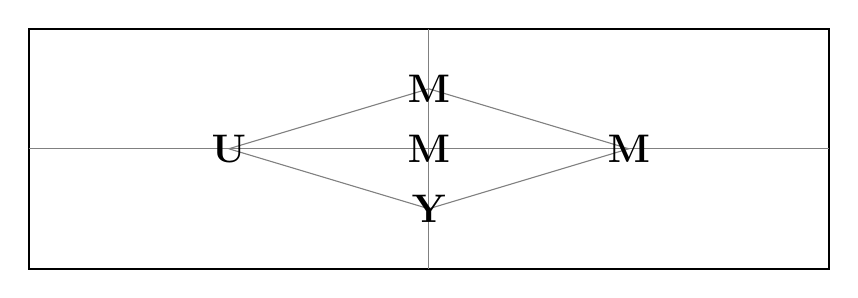
\begin{tikzpicture}[x=1in,y=0.3in]\bf\Large
  \draw[thick] (0,0) rectangle (4,4);
  \draw[color=gray,thin] (0,2) -- (4,2);
  \draw[color=gray,thin] (2,0) -- (2,4);
  \draw[color=gray,thin] (1,2) -- (2,1) -- (3,2) -- (2,3) -- (1,2);
  \node at (2,3) {M};
  \node at (1,2) {U};
  \node at (2,2) {M};
  \node at (3,2) {M};
  \node at (2,1) {Y};
\end{tikzpicture}
\end{center}
